\documentclass{article}
\usepackage{array}
\usepackage{caption}
\usepackage{fancyhdr}
\usepackage{graphicx}
\usepackage{hyperref}
\usepackage{lastpage}
\usepackage{lmodern}
\usepackage[utf8]{inputenc}
\usepackage{polski}

\graphicspath{ {./images/} }
\urlstyle{same}

\title{Specyfikacja Projektu ,,Expert4Home''}
\author{K. Dąbrowski, J. Grygiel, S. Kalisz\\
K. Malinowski, P. Piętka, B.Zdrojewski}
\date{Wersja 1.0\\\today}

\pagestyle{fancy}
\fancyhf{}
\lhead{Specyfikacja Projektu ,,Expert4Home''}
\rhead{Wersja 1.0}
\rfoot{\thepage \hspace{1pt} / \pageref{LastPage}}

\begin{document}

	\maketitle
	\thispagestyle{empty}  
	\newpage
  
	\section{Wstęp} 
  
	\subsection{Cel dokumentu}
	todo bz
  
	\subsection{Cel projektu}
	todo bz
  
	\subsection{Użytkownicy końcowi}
	todo bz
  
	\section{Architektura systemu}
  
  \subsection{Aktorzy}
	% todo kd definicja użytkownika, klienta, specjalisty
	Osoby korzystające z aplikacji będą mogły grać rolę różnych aktorów podczas interakcji z systemem w zależności od celu, który chcą osiągnąć.
	Oznacza to, że ta sama osoba może raz wystąpić w roli eksperta oferującego swoje usługi, a innym razem skorzystać z systemu jako klient szukający wykonawcy zlecenia.

	\subsubsection*{Lista przewidzianych aktorów}
	\begin{itemize}
		\item Ekspert -- Osoba posiadająca wiedzę i umiejętności w danej dziedzinie pozwalające na świadczenie usług innym,
		\item Klient -- Osoba szukająca wykonawcy usług
		\item Stały klient -- Klient, który nawiązał wielokrotną w spółpracę z \textbf{konkretnym ekspertem}. Ma on dostęp do dodatkowych benefitów udzielonych przez eksperta
		\item Administrator -- Osoba mająca dodatkowe uprawnienia dzięki którym może wypływać na działanie systemu dla zwykłych użytkowników
	\end{itemize}
	
  \subsection{Przypadki użycia}
  Diagram przypadków użycia przedstawia rysunek \ref{fig:ucDiagram}.

  \begin{figure}[h]
	  \centering
	  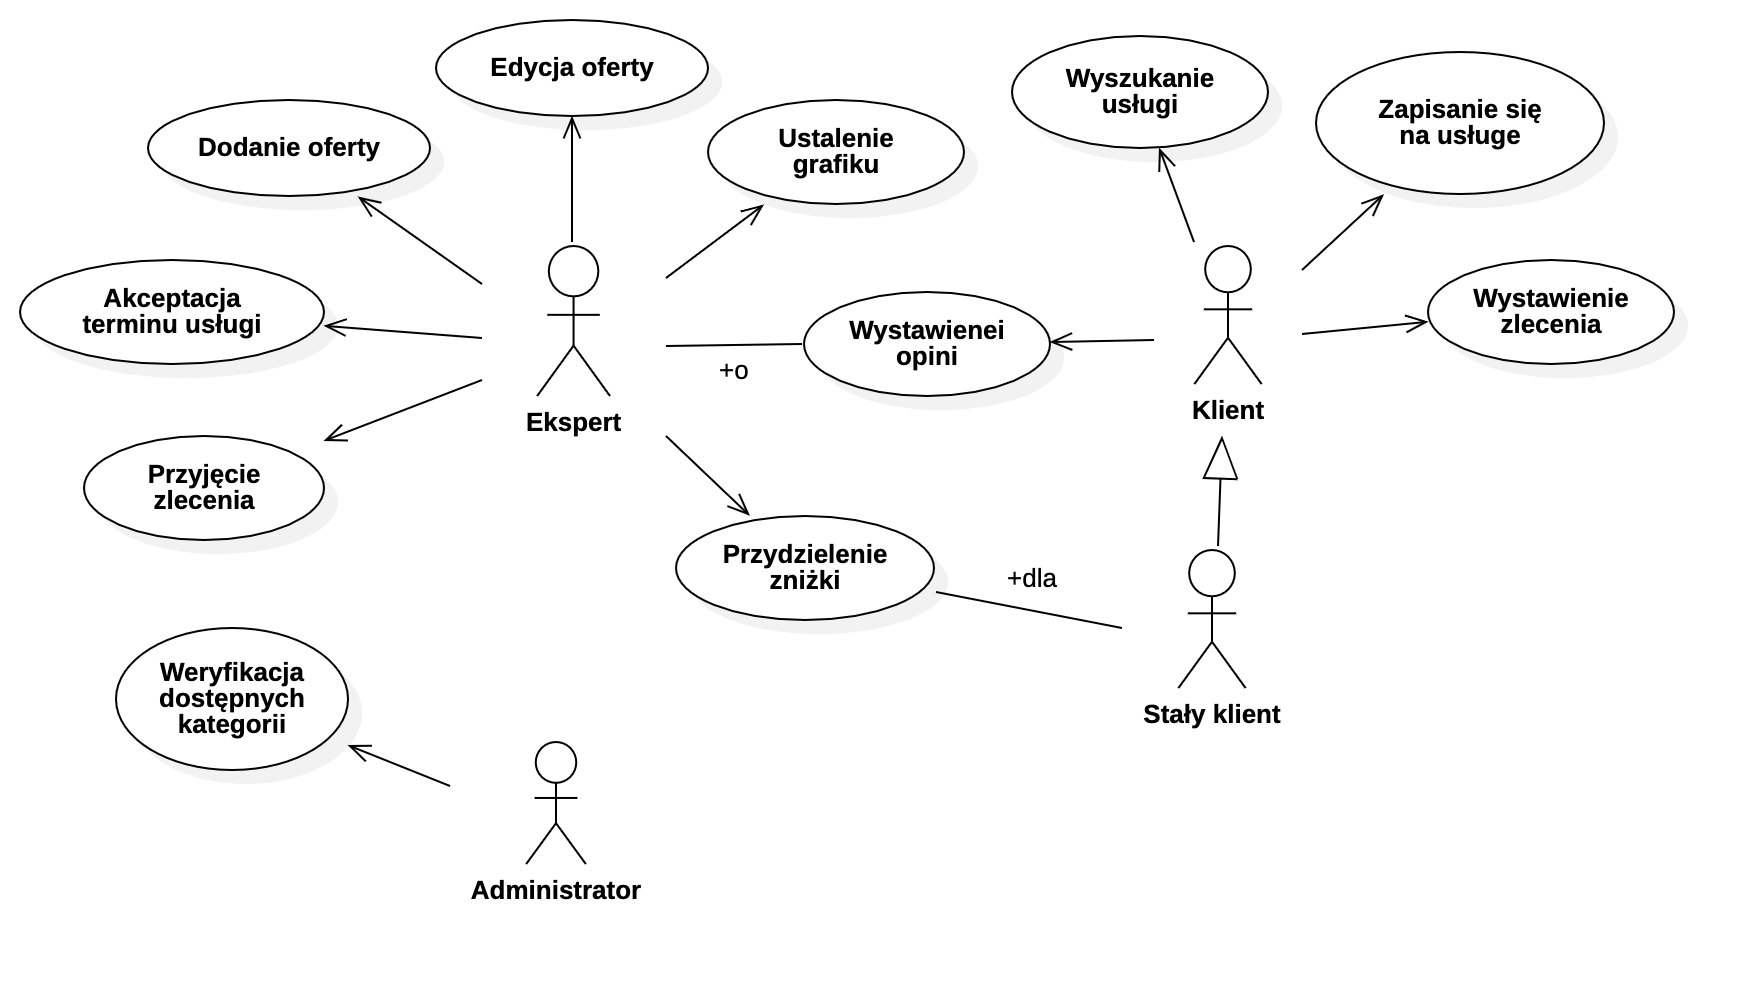
\includegraphics[width=0.8\textwidth{}]{use_case_diagram.png}
	  \caption{Diagram przypadków użycia}
	  \label{fig:ucDiagram}
  \end{figure}
  
  \subsection{Diagramy sekwencji}
	todo kd tak jak na uml'u, na jednym diagramie (użyć \url{https://draw.io}, projekt zapisać w schemes, obraz wyeksportować do images, obraz wstawić z podpisem) przedstawić proces wyszukania specjalisty, dodania zgłoszenia, zaakceptowania zgłoszenia przez specjalistę i wystawienia komentarza, na podstawie zdjęć ze slackowego hash tag frontend (zdaję sobię sprawę, że wyciągnięcie procesu ze zdjęć widoków może być nieoczywiste, więc w razie czego pisz do bz/jg/sk)
  
	\section{Interfejs użytkownika}
  
	\subsection{Ekran główny}
	todo jg przerysować w \url{https://draw.io} ze slackowego hash tag frontend, zapisać projekt do schemes, wyeksportować obraz do images, wstawić obraz tutaj z podpisem
	
	\subsection{Ekran wyszukiwania specjalisty}
	todo jg przerysować w \url{https://draw.io} ze slackowego hash tag frontend, zapisać projekt do schemes, wyeksportować obraz do images, wstawić obraz tutaj z podpisem
	
	\subsection{Ekran profilu specjalisty}	
	todo jg przerysować w \url{https://draw.io} ze slackowego hash tag frontend, zapisać projekt do schemes, wyeksportować obraz do images, wstawić obraz tutaj z podpisem	
	
	\subsection{Dialog zgłoszenia}	
	todo sk przerysować w \url{https://draw.io} ze slackowego hash tag frontend, zapisać projekt do schemes, wyeksportować obraz do images, wstawić obraz tutaj z podpisem	
	
	\subsection{Ekran zgłoszeń klienta}
	todo sk przerysować w \url{https://draw.io} ze slackowego hash tag frontend, zapisać projekt do schemes, wyeksportować obraz do images, wstawić obraz tutaj z podpisem
	
	\subsection{Ekran zgłoszeń specjalisty}
	todo sk przerysować w \url{https://draw.io} ze slackowego hash tag frontend, zapisać projekt do schemes, wyeksportować obraz do images, wstawić obraz tutaj z podpisem  
  
	\section{Szczegóły implementacji}  
  
	\subsection{Środowisko deweloperskie}  
	todo pp windows/linux, intelij, wersje
  
	\subsection{Zastosowane technologie}

	\subsubsection{Front-end}	
	todo jg+sk react
	
	\subsubsection{Back-end}	
	todo kd+km+pp springboot, mysql, nginx	
	
	\subsubsection{Kontrola wersji}
	todo bz git
	  
	\subsubsection{Wdrożenie oprogramowania}
	todo km+pp docker
	  
	\subsection{Plan testów}
	todo km jednostkowe, integracyjne, sam wiesz lepiej
 
	\section{Szczegóły organizacji prac}  
 
	\subsection{Harmonogram prac}
	todo bz
 
	\subsection{Metodyka wytwarzania oprogramowania}
	todo sk scrum, kanban
	
	\subsection{Zastosowane narzędzia}
	todo kd azure devops, slack
 
\end{document}